\begin{center}
\textsc{\Large Laboratorio 11}~\\
{\large Vídeo Juegos, Diseño, Programación}~\\
\emph{Arte, Assets, Texturas y Modelos}
\end{center}

\section{Pre-Laboratorio}
\begin{itemize}
\item Investigar:
\begin{enumerate}
  \item Game Asset Management y Control de Versiones.
  \item Licencias y derechos de autor.
\end{enumerate}
\item De algún juego que conozca analice.
\begin{enumerate}
  \item Arte del juego, investigue arte conceptual de este juego.
  \item ¿Es el arte del juego congruente con los conceptos de arte?
  \item ¿Existe cierta relación entre el ambiente y arte del juego y su genero? ¿De que forma?
\end{enumerate}
\end{itemize}

\setlength\intextsep{0pt}
\begin{wrapfigure}[7]{r}{0.35\linewidth}
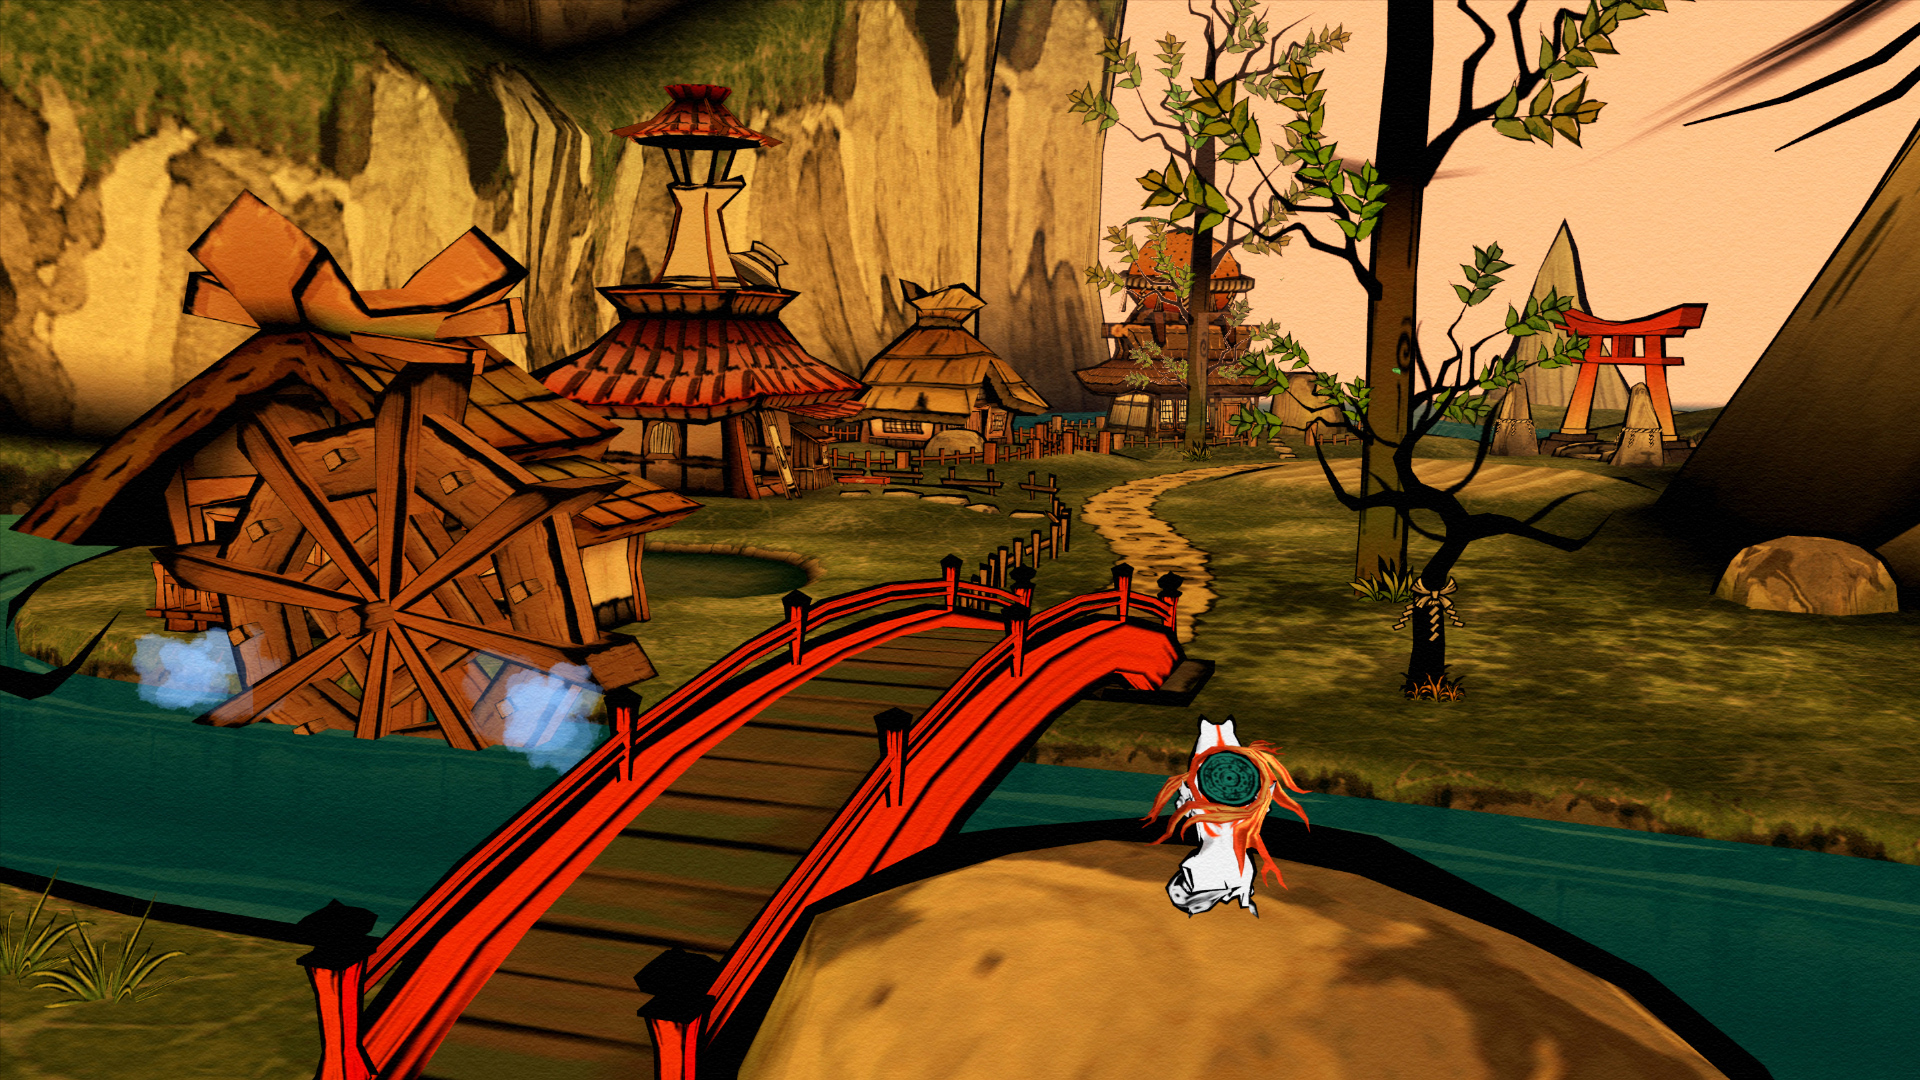
\includegraphics[width=\linewidth]{media/okamips2.jpg}
\caption{\emph{Okami} \cite{okami} es un juego con arte inspirado en sumi-e \cite{sumie}.}
\label{fig:particles}
\end{wrapfigure}
\section{Introducción}
Buen arte se ha convertido en una forma de de juzgar los vídeo juegos. Un inmensa mayoría compra y gana interés en algún vídeo juego a partir de como estos se ven, esto es una reacción lógica ya que desde una tienda virtual o física o a través de vídeos o tomas de pantallas no se puede evaluar el gameplay del juego en cuestión \cite[p.~171]{bobbatesgamedesign}.

Los artistas afectan ahora una inmensa parte del diseño del juego, desde el diseño de la interfaz de juego hasta hasta el ambiente general presentado en el universo del juego y los efectos especiales. La creación de arte ha aumentando en complejidad a través de los años y el crecimiento de los vídeo juegos como una industria, de tal forma las herramientas de creación de arte también cada vez son mas complejas.
\section{Actividad}
\todo[inline]{Por hacer.}